\chapter{Metodologia}
\label{chap:MatMet}

\section{Divergência em avaliação de similaridade de formas}


A avaliação de similaridade entre formas a partir de medidas de divergência requer que as informações das assinaturas, abordadas na Seção \ref{sec:Assinatura} do Capítulo \ref{chap:contour}, sejam tratadas como variáveis aleatórias e que suas distribuições de probabilidade sejam estimadas. 

A  Figura \ref{fig:metodo_distancia} ilustra como divergentes podem ser aplicados na avaliação da similaridade entre duas formas A e B. No método em questão, as distribuições de probabilidade de quatro assinaturas distintas dos contornos das formas são estimadas, através de histogramas, para em seguida se calcular as medidas de divergência. Uma medida de similaridade é então obtida  a partir da média ponderada das medidas de divergência.

\begin{figure}[h!]
  \caption{\label{fig:metodo_distancia} Método para avaliação da similaridade entre duas formas A e B utilizando distância estocástica e histogramas das assinaturas do contorno das formas.}
  \centering
  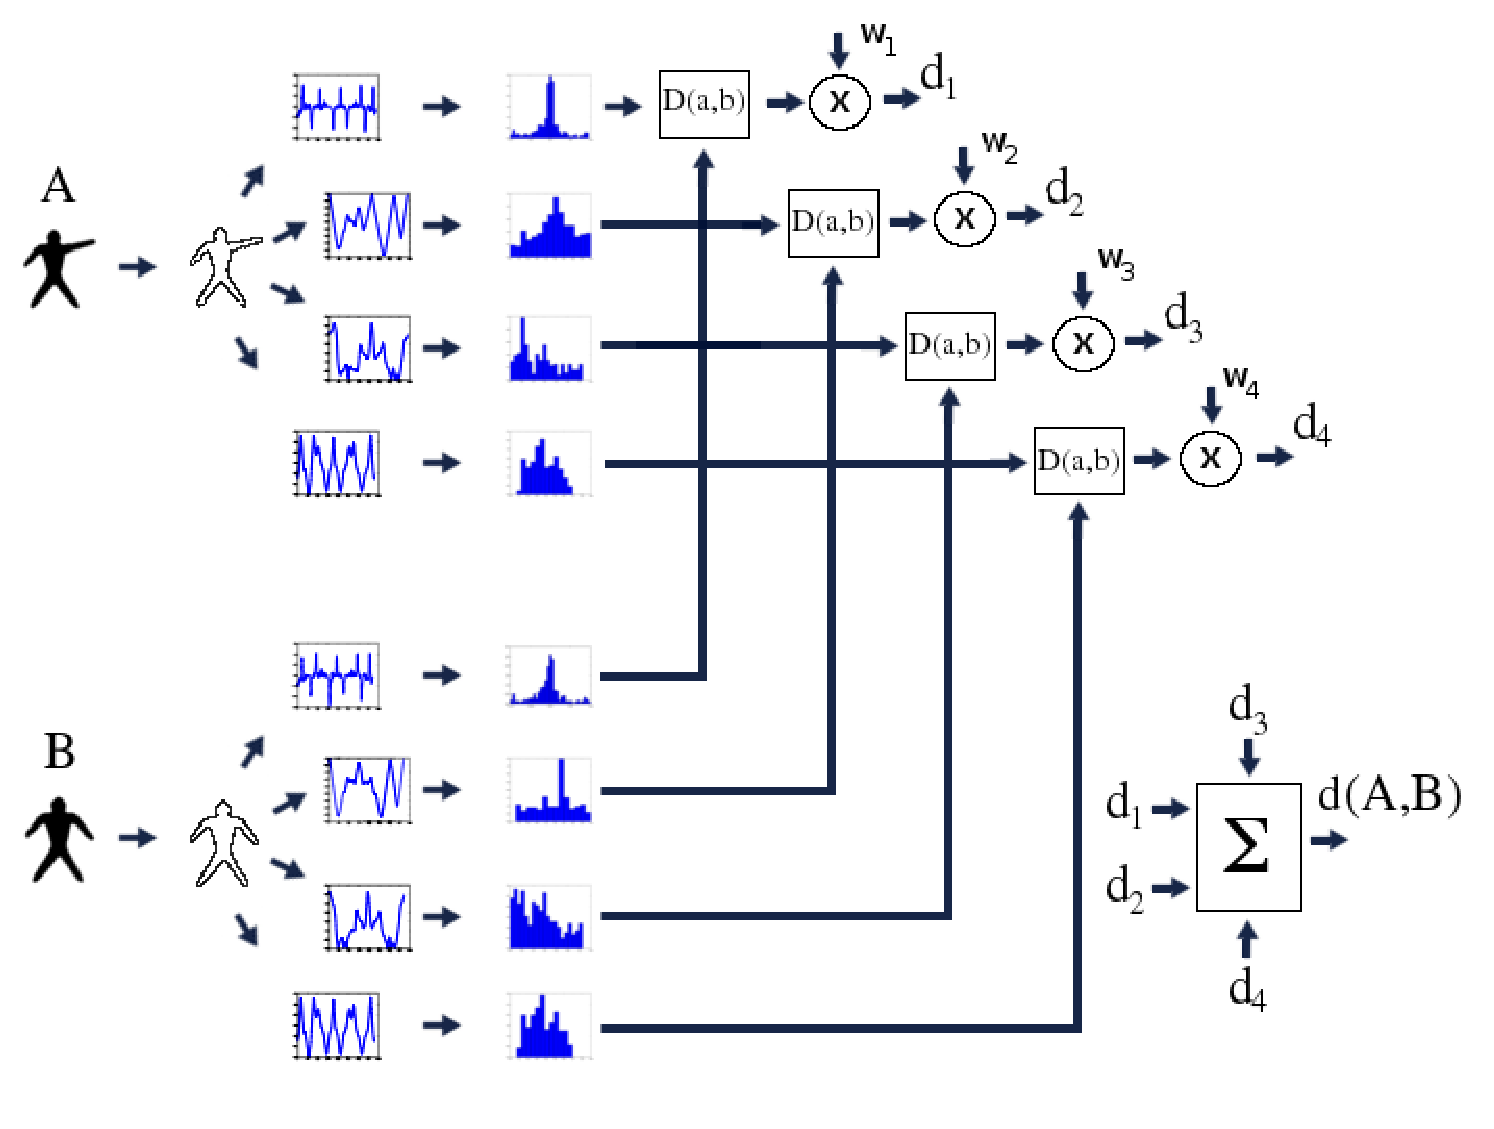
\includegraphics[width=0.85\textwidth]{figura_metodo.eps}
\end{figure}


\begin{comment}
\subsection{Visualizaçâo de dados}

A Figura \ref{fig:metodo_4} ilustra o método que empregamos na avaliação da capacidade discriminativa dos descritores de formas através das técnicas de visualização dos dados apresentadas.

\begin{figure}[h!]
  \caption{\label{fig:metodo_4} Método de avaliação de descritores multiescala do contorno de formas. (a) Base de imagens. (b) Extração de características. (c) Descritores de formas. (d) Análise de similaridade a partir da matriz-U. (e) Avaliação de agrupamentos a partir da medida silhouette.}
  \centering
  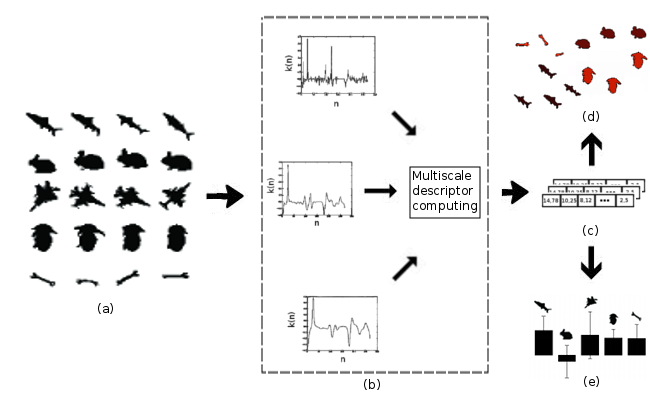
\includegraphics[width=0.75\textwidth]{metodo_v4.png}
\end{figure}

O primeiro passo consiste em realizar a extração de características num conjunto de formas binárias rotuladas (Figura \ref{fig:metodo_4}a e Figura \ref{fig:metodo_4}b) com o método de descrição sob análise. Como resultado temos um conjunto de descritores, ou vetores de características, das referidas formas (Figura \ref{fig:metodo_4}c). 

A avaliação de qualidade dos descritores se dá qualitativamente e quantitativamente. Na avaliação qualitativa (Figura \ref{fig:metodo_4}d) utilizamos a rede auto-organizável de Kohonen para obtenção da matriz de distâncias unificada, ou matriz-U. Essa última é empregada como ferramenta de visualização dos dados, o que possibilita identificar como o método de descrição sob avaliação agrupa as formas. 

Na avaliação quantitativa (Figura \ref{fig:metodo_4}e) utilizamos os rótulos e os vetores de características das formas para calculamos a medida de avaliação de agrupamentos \emph{Silhouette} \cite{Rousseeuw:1987}. Valores médios dessa medida, por classe de formas, indica a habilidade dos descritores em discriminar formas que pertençam a classes distintas e de agrupar formas que pertençam a uma mesma classe.
\end{comment}
\section{Ajuste de parâmetros}
A metodologia proposta para escolha de parâmetros do descritor segue o esquema da Figura \ref{fig:Avaliacao}. Essa metodologia melhora a representação do descritor utilizando métodos de otimização evolutivos para minimizar uma função custo que corresponde a mediana do erro absoluto da silhouette dos descritores ($MAD$). O que motivou a escolha dessa função custo é sua robustez a valores extremos \cite{Rousseeuw:1987:2}, sendo sua equação 

\begin{equation}
\label{eq:mad}
MAD = \operatorname{mediana}\big(|s_i - 1|_{i =1,\:2,\:\cdots,\:L}\big)\text{,}
\end{equation}

\noindent aonde $S = \{s_1,s_2,\cdots,s_L\}$ é o conjunto das \emph{silhouettes} calculadas para $L$ descritores de forma. Os operadores $|.|$  e {$mediana ( )$} retornam o valor absoluto e a mediana de um conjunto de valores, respectivamente.

A Silhouette \cite{Rousseeuw:1987} é uma medida de qualidade de agrupamentos que indica o grau de afinidade de uma amostra  a um agrupamento, levando em conta as distâncias médias entre-classes e intra-classes de um objeto $i$ atribuído a uma dada classe $A$. Logo, esta métrica é definida como 
\begin{equation}
s_i = \frac{b_i - a_i}{\max{(a_i,b_i)}} \in [-1,1],
\end{equation}

\noindent sendo $a_i$ a dissimilaridade média entre o objeto $i$ e os demais objetos pertencentes a mesma classe de $a_i$ e $b_i$ é a dissimilaridade média do objeto $i$ e a classe vizinha mais próxima de $i$, excluída sua própria classe. 

Essa métrica pode assumir valores no intervalo $[-1,1]$, sendo que valores negativos indicam que o grau de pertencimento de um objeto à classe que este fora atribuído é baixo. Já valores positivos indicam que o grau de pertencimento de um objeto à classe que este fora atribuído é alto. Um valor de silhouette próximo de zero indica que o objeto está na fronteira entre duas classes e que há, portanto, um grau de incerteza a respeito de qual classes este pertence.

Os valores da função objetivo $MAD$ assume valores no intervalo $[0,2]$. De forma análoga a silhouette, um valor igual a zero desta função indica que a estrutura dos clusters é perfeita, enquanto que valores próximos de $2$ indicam que a estrutura dos clusters é deficiente, com baixa similaridade entre os objetos de mesma classe ou alta similaridade entre os objetos de classes distintas.

A Figura  \ref{fig:Avaliacao} ilustra como a metodologia proposta ajusta os parâmetros do descritor multiescala, bem como esta avalia a qualidade do descritor obtido com os parâmetros otimizados. Primeiramente, é amostrado na base de folhas um sub-conjunto das formas para, em seguida, realizar o procedimento de otimização e encontrar o melhor conjunto de parâmetros de escala  $\boldsymbol{\sigma}_{otim} = (\sigma_1,\:\sigma_2,\:\cdots,\:\sigma_k)$ do descritor multiescala que minimize a função custo da Equação \ref{eq:mad}. Então, utilizando-se as escalas encontradas realiza-se, com o descritor multiescala, a extração de características de toda a base de folhas.

\begin{figure*}
\centering
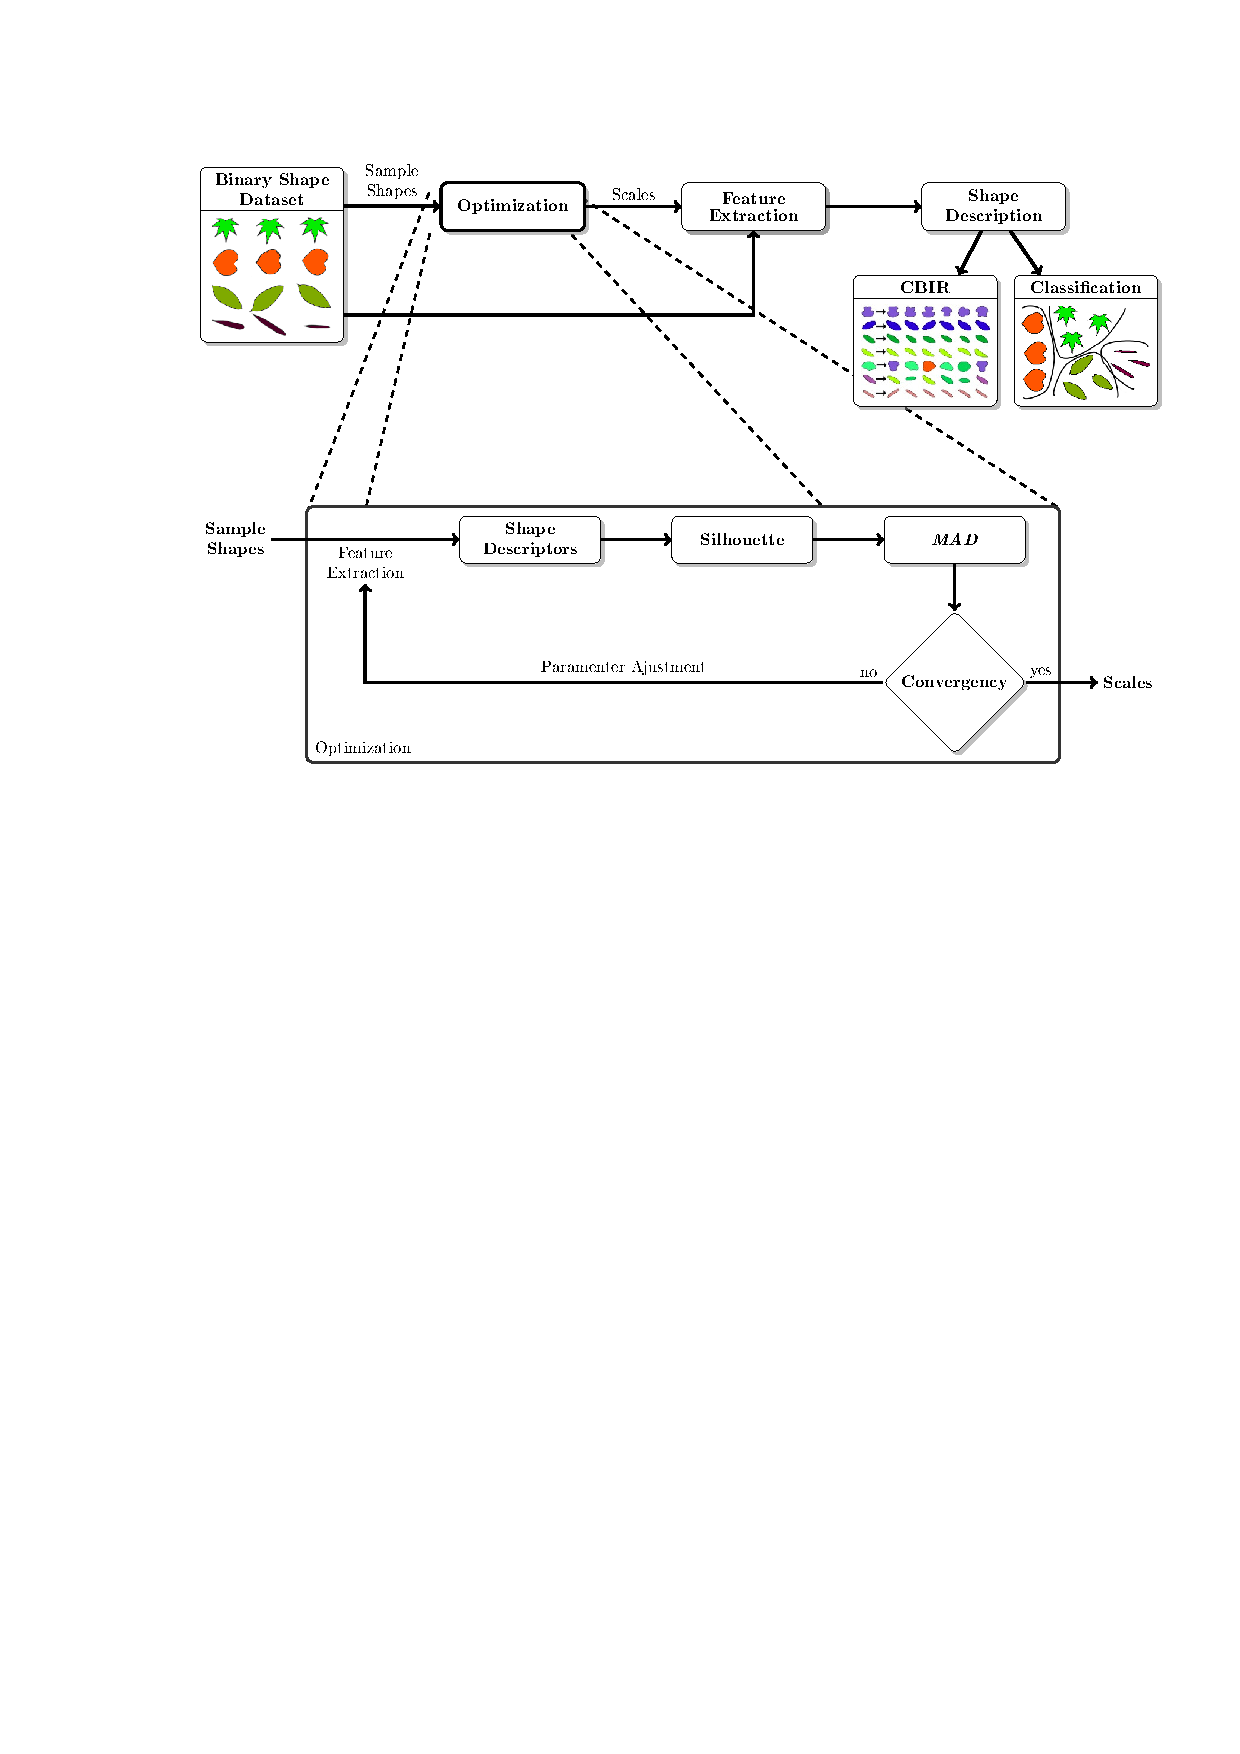
\includegraphics[width=\textwidth,trim = 14mm 164mm 0mm 24mm,clip]{Final_Flux.pdf}
\caption{The proposed approach for evolutionary optimization of a multiscale shape descriptor.} 
\label{fig:Avaliacao}
\end{figure*}

O desempenho do descritor, em termos de agrupamento das formas, é avaliado qualitativamente e quantitativamente. Na avaliação qualitativa dois algoritmos de visualização de dados são utilizados: o mapa auto-organizável de Kohonen \cite{Kohonen:2001} e o \textit{multidimensional scaling} \cite{cox:2000}. Esses algoritmos produzem projeções bi-dimensionais das descrições das formas da base de folhas, provendo uma representação gráfica que possibilita a análise da qualidade dos agrupamentos. Assim, consegue-se inferir o quão eficaz o descritor é em organizar espacialmente as formas. Já na avaliação quantitativa são analisadas métricas de avaliação obtidas em experimentos de classificação supervisionada (precisão e revocação), de recuperação de formas (bulls-eye) e a medida silhouette \cite{Rousseeuw:1987} média por classe. 

A silhouette média por classe avalia tanto a coesão como a separação das classes através da distância entre os vetores de características. Já as métricas de precisão e revocação são medidas clássicas na avaliação do desempenho de descritores em experimentos de classificação supervisionada. Na classificação supervisionada, os classificadores utilizados foram Naive Bayes (NB) \cite{Fukunaga:1990}, \emph{K}-vizinhos próximos (Knn, $K = 5$) \cite{Fukunaga:1990,Webb:2002},  o discriminante linear de Fisher (LDA) \cite{Webb:2002} e o discriminante quadrático (QDA) \cite{Fukunaga:1990}.  Antes da classificação com os classificadores NB e \emph{Knn} foi utilizado o discriminante linear de Fisher para transformar os dados \cite{Webb:2002}. Já para classificação com os classificadores LDA e QUA aplicou-se a análise das componentes principais para descorrelacionar os dados. Os experimentos realizados de recuperação de imagens pelo conteúdo visam avaliar o desempenho dos descritores de formas e das medidas de similaridade estudadas neste trabalho. As metodologias utilizadas nesses experimentos são as mesmas encontradas em diversos trabalhos de recuperação de formas da literatura.

Foram realizados experimentos em duas bases de imagens de formas binárias: a Kimia, de 99 formas, e a MPEG-7 CE-Shape-1 de 1400 formas. Ambas as bases estão apresentadas no Apêndice deste trabalho.

A  Figura \ref{fig:metodo_cbir} ilustra a metodologia dos experimentos de recuperação de formas.  Primeiramente realiza-se a extração de características das formas da base de imagens de formas binárias com o método de descrição sob avaliação. O mesmo processo de extração de características é aplicado a imagem de uma forma de consulta. Esse processo resulta numa base de dados com os vetores de características associados às formas utilizadas no experimento. 

Com a medida de similaridade avalia-se o grau de correspondência existente entre o vetor de características da forma de consulta e os vetores associados a cada uma das formas da base. Tem-se assim como resultado uma lista de imagens recuperadas em ordem decrescente de similaridade à forma de consulta. Todo esse processo é realizado repetidamente tomando-se cada forma da base de imagens como forma de consulta e recuperando-se as demais.

\begin{figure}[h!]
  \caption{\label{fig:metodo_cbir} Metodologia empregada para os experimentos de recuperação de formas pelo conteúdo.}
  \centering
  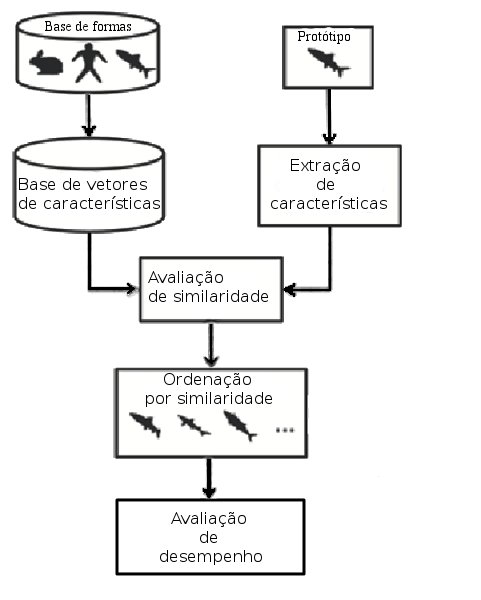
\includegraphics[width=0.55\textwidth]{Metodologia1.jpg}
\end{figure}

Na avaliação do desempenho dos experimentos duas medidas são utilizadas: o número total de acertos por posição recuperada e a medida Bull-eye.

A primeira medida consiste no número total de ocorrências de formas da mesma classe que a forma de consulta em cada posição recuperada.  Em diversos trabalhos de recuperação de formas pelo conteúdo o número total de acertos por posição recuperada é calculado para a base Kimia-99 \cite{Bernier:2003}. Tendo esta base 99 formas, igualmente distribuídas em 9 classes, são realizadas 99 recuperações das 11 formas mais similares à imagem de consulta. Como resultado espera-se obter um total de 99 formas recuperadas corretamente para cada posição recuperada.

A medida Bull-eye também é utilizada na literatura para a comparação de diferentes métodos de recuperação de formas. Essa medida é calculada para a base MPEG-7 CE-Shape-1 da seguinte maneira: tomando-se cada forma dessa base de imagens como elemento de consulta, contabiliza-se o número de recuperações pertencentes a mesma classe da forma de consulta dentre as 40 primeiras posições recuperadas. Como resultado calcula-se a percentagem da quantidade máxima de recuperações corretas possíveis de se alcançar, sendo esta última quantidade $28000 = 1400\text{ formas} \times 20\text{ recuperações corretas poro forma}$. 
 

\section{Optimization methods}

This paper investigates three optimization algorithms to search for the best solution that minimizes the objective function MAD: the simulated annealing (SA), differential evolution (DE) \cite{Storn:1007} and particle swarm (PSO) \cite{Yuhui:1998}. 

Simulated annealing is a classical probabilistic optimization procedure that simulates the thermodynamic process of material heating and cooling. This algorithm encompasses a temperature variable such that the higher it is, the higher is the probability of the algorithm to accept worse solutions as it explores the solution space. Thus, the temperature variable decreases exponentially as the algorithm iterates and therefore the probability to accept the worse solutions decreases over time. Then, the algorithm converges to an optimal solution. Particularly, the implemented algorithm embodies a mechanism to disturb the current solution which consists in adding or subtracting,  with a given probability $P_r$, a value from each coordinate of the current solution. In fact, this value is drawn from a normal distribution, with zero mean and variance, i.e., $\kappa.v_i.(1+COST(v))$, where $\kappa = 0.6$, $v_i$ is the $i_{th}$ coordinate of the current solution and $COST(v)$ is the fitness. 

\begin{comment}
\begin{algorithm}[ht]
\caption{Simulated Annealing}
\label{alg:sa}
\begin{algorithmic}
\Require $N\text{,}\:M\text{,}\:T_0\text{,}\:P\text{,}\:L> 0$, $:\alpha\text{,}\:\kappa\text{,}\:P_r \in [0,1]$, $\:COST$.
\Ensure The best found solution that minimizes $COST$.

\Function{DISTURB}{$\boldsymbol{v}$}
\State $f \gets$ \Call{$COST$}{$\boldsymbol{v}$}
\For{$i = 0,\:1,\:\cdots,\:M-1$} 
\If {$P_r > U(0,1)$}
\State $aux \gets v[i]$
\State $v[i] \gets v[i]+ \kappa.(1+f).\mathcal{N}(0,1).v[i]$
\If {$v[i] \notin [0.125,125.5]$}
\State $v[i] \gets aux$
\EndIf
\EndIf
\EndFor
\State \Return $\boldsymbol{v}$
\EndFunction

\State $i \gets 1$, $n \gets 0$,$T \gets T_0$
\For{$j = 0,\:1,\:\cdots,\:M-1$} 
\State $s[j] \gets U(0.125,125.5)$
\EndFor
\State $fit \gets$ \Call{$COST$}{$\boldsymbol{s}$} 
\Repeat
\State $\boldsymbol{s_d} \gets$ \Call{$Disturb$}{$\boldsymbol{s}$}
\State $\delta \gets$ \Call{$COST$}{$\boldsymbol{s_d}$}$- fit$ 
\If {$\delta < 0$ or $\exp{(\frac{\delta}{T})} > U(0,1)$}
\State $\boldsymbol{s} \gets \boldsymbol{s_d}$,$fit \gets $ \Call{$COST$}{$\boldsymbol{s_d}$}
$n \gets n + 1$
\EndIf
\State $i \gets i + 1$
\Until{$i > P$ or $n > L$}
\State $T \gets \alpha.T$
\end{algorithmic}
\end{algorithm}
\end{comment}

The differential evolution algorithm iteratively evolves a population of $N$ vectors of candidate solutions and it produces disturbed versions of each population solution by using a disturbance vector. Here, we employ the  \emph{DE/rand/1} strategy introduced by \cite{Storn:1996},  which is a modified version of DE that computes the disturbance vector according to equation:
\begin{equation}
\boldsymbol{d} = \boldsymbol{\sigma_1} + \beta.(\boldsymbol{\sigma_2} - \boldsymbol{\sigma_3}),
\end{equation}

\noindent where $\boldsymbol{\sigma_1}$, $\boldsymbol{\sigma_2}$ and $\boldsymbol{\sigma_3}$ are three randomly selected distinct candidate solutions in the population, which are also different from the current solution to be disturbed.  The $\beta$ parameter is an amplification factor of the difference between $\boldsymbol{\sigma_2}$ and $\boldsymbol{\sigma_3}$. The disturbance occurs in each coordinate of the current solution, via a cross-over mechanism with probability $P_r$. Then, the disturbed solution replaces the current one in population if it has a better fitness, otherwise the algorithm keeps the current solution. 
In this paper, we have tuned the algorithm parameters ($N$,$\beta$,$P_r$) by following the guidelines in \cite{Storn:1996} and performing several tests. Finally,  we have approached the proposed optimization problem with the  parameter set: $N = 100$, $\beta = 0.56$ and $P_r = 0.3$.

\begin{comment}
\begin{algorithm}[ht]
\caption{Differential evolution optimization}
\label{alg:de}
\begin{algorithmic}
\Require $N\text{,}\:M > 0$, $\:\beta\text{,}\:P_r \in (0,1]$, $\:COST$
\Ensure The best found solution that minimizes $COST$
\For{$i = 0,\:1,\:\cdots,\:N-1$}
\For{$j = 0,\:1,\:\cdots,\:M-1$}
\State $\boldsymbol{pop}[i][j] \gets U(0.125,125.0)$
\EndFor
\EndFor

\For{$j = 0,\:1,\:\cdots,\:1250$}
\For{$i = 0,\:1,\:\cdots,\:N-1$}
\State Select in $\boldsymbol{pop}$ three random distinct candidate solutions ($\boldsymbol{\sigma_a}$, $\boldsymbol{\sigma_b}$ and $\boldsymbol{\sigma_c}$) that differ from $\boldsymbol{pop}[i]$
\State $\boldsymbol{d} \gets \boldsymbol{\sigma_a} + \beta.(\boldsymbol{\sigma_b} - \boldsymbol{\sigma_c})$
\For{$k = 0,\:1,\:\cdots,\:M-1$}
\If{$\boldsymbol{d}[k] \notin [0.125,125.0]$}
\State $\boldsymbol{d}[k] \gets U(0.125,125.0)$
\EndIf
\EndFor
\State $\boldsymbol{c} \gets \boldsymbol{pop}[i]$
\State $k \gets U(0,M-1)$
\State $c[k] \gets d[k]$
\For{$k = 0,\:1,\:\cdots,\:M-1$}
\If {$U(0,1) \leq P_r$}
  \State $c[k] \gets d[k]$
\EndIf
\EndFor

\If {\Call{$COST$}{$\boldsymbol{c}$} $<$ \Call{$COST$}{$\boldsymbol{pop}[i]$}}
 \State $\boldsymbol{pop}[i] \gets \boldsymbol{c}$
\EndIf
\EndFor
\EndFor
\end{algorithmic}
\end{algorithm}
\end{comment}

Particle swarm optimization is a bio-inspired algorithm that evolves a population of $N$ solutions (particles) that move in the search space with a given velocity. This algorithm keeps track of the best positions attained by each particle (\emph{bpp}) and the best global position obtained by all particles (\emph{bgp}) of the swarm.  At each iteration, PSO corrects the particle velocities in the search space influenced by two attraction factors $c_1$ and $c_2$. The first factor  controls the tendency of the particle to search around its own best position (bpp) and the second one controls the tendency to move towards the best global position (bgp) found.  In order to guarantee that PSO converges to a global minimum, the particles decelerate exponentially along iterations with an inertia factor $\omega$ \cite{Yuhui:1998}. Here,  we have tuned the PSO parameters to $N = 25$, $\omega = 0.95$ and $c_1 = c_2 = 2$. It is worth noting that these values satisfy the convergence criteria for this optimization algorithm as described in \cite{Jiang20078}.
\begin{comment}
\begin{algorithm}[ht]
\caption{Particle Swarm Optimization}
\label{alg:pso}
\begin{algorithmic}
\Require $N\text{,}\:M > 0$,  $\:\omega \in (0,1]$, $\:c_1\text{,}\:c_2 \in R^+ $, $\:COST$
\Ensure The best found solution that minimizes $COST$
\For{$i = 0,\:1,\:\cdots,\:N-1$}
\For{$j = 0,\:1,\:\cdots,\:M-1$}
\State $pop[i][j] \gets U(0.125,125.5)$ 
\State $v[i][j] \gets U(0.125,125.5)$
\EndFor
\State $fit[i] \gets$ \Call{$COST$}{$\boldsymbol{pop}[i]$}
\State $\boldsymbol{bpp}[i] \gets \boldsymbol{pop}[i]$ 
\EndFor
\State $\boldsymbol{bgp} \gets \boldsymbol{bpp}[argmin(\boldsymbol{fit})]$
\For{$i = 0,\:1,\:\cdots,\:1250$}
\For{$j = 0,\:1,\:\cdots,\:N-1$}
\State $\boldsymbol{v}[j] \gets \omega.\boldsymbol{v}[j]$
\State $\boldsymbol{v}[j] \gets \boldsymbol{v}[j] + c1.U(0,1).(\boldsymbol{pop}[j] - \boldsymbol{bpp}[j])$
\State $\boldsymbol{v}[j] \gets \boldsymbol{v}[j] + c2.U(0,1).(\boldsymbol{pop}[j] - \boldsymbol{bgp})$
\State $\boldsymbol{pop}[j] \gets \boldsymbol{pop}[j] + \boldsymbol{v}[j]$
\For{$k = 0,\:1,\:\cdots,\:M-1$}
\If{$pop[j][k] \notin [0.125,125.0]$}
\State $pop[j][k] \gets U(0.125,125.0)$
\EndIf
\EndFor
\State $fit[j] \gets$ \Call{$COST$}{$\boldsymbol{pop}[j]$}
\If {$fit[j] <$ \Call{$COST$}{$\boldsymbol{bpp}[j]$}} 
\State $\boldsymbol{bpp}[j] \gets \boldsymbol{pop}[j]$
\EndIf
\If {\Call{$COST$}{$\boldsymbol{bpp}[j]$} $<$ \Call{$COST$}{$\boldsymbol{bgp}$}}
\State $\boldsymbol{bgp} \gets \boldsymbol{bpp}[j]$
\EndIf
\EndFor
\EndFor
\end{algorithmic}
\end{algorithm}
\end{comment}

\begin{comment}
\subsection{Self-organizing map and the U-matrix}

The self-organizing map, or SOM network \cite{Kohonen:2001}, is a neural network that performs nonlinear reduction of high-dimensional data by projecting it into a low-dimensional space. This method is an exploratory data analysis tool that has been used for image visualization \cite{Strong2011774}, cluster learning \cite{Kuroiwa200031} and texture classification \cite{595364}. 

A SOM network represents structural features of input data in a low-dimensional lattice. In fact, this tool displays data features in the lattice by using a neighborhood criterion in order to preserve structure of the input space.  According to \cite{Ultsch:1990}, the direct usage of this network output is not suitable for cluster analysis purposes.  The SOM network arranges clusters in different regions, although the distances among data points are uniformly distributed. To overcome this drawback, Ultsch and Siemon \cite{Ultsch:1990} developed a two-dimensional projection method, namely the unified distance matrix, i.e., the U-matrix. The U-matrix displays the local distance structure of a topology-preserving projection of a high-dimensional data set \cite{Ultsch:1990}.

\begin{figure}[!ht]
\centering
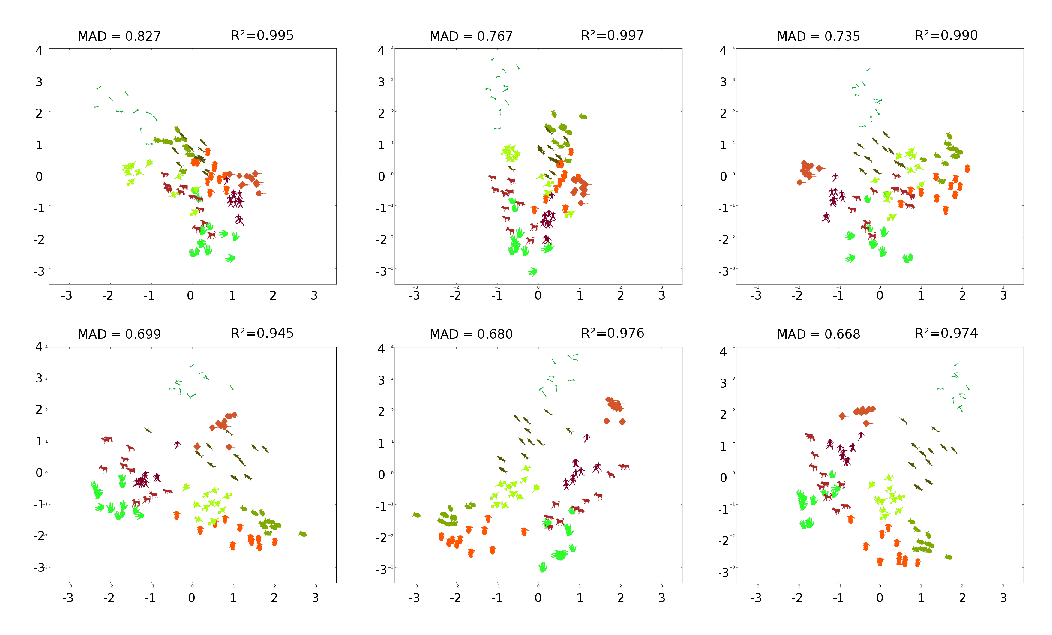
\includegraphics[width=0.75\textwidth]{fig4.eps}
\caption{\label{fig:projkimia99}U-matrices for shapes of MPEG7 CE-Shape-1 data set.}
\end{figure}

Figure \ref{fig:projkimia99} shows the U-Matrix for shapes of the MPEG-7 CE-Shape-1 data set \cite{855850}. The central image is the result of the whole data set described by the optimized NMBE.  The four images in the corners are details of the central image.
This visualization tool identifies how well NMBE describes subtle details from shapes of the same cluster and different clusters. In the detail images, we can observe the boundaries (in grey) which separate the well-defined shape clusters (e.g. clusters in the top-left corner image). Well-defined clusters are the ones with the lowest within-class and highest inter-class distances.

\section{Multidimensional Scaling (\emph{MDS})}
The multidimensional scaling \cite{cox:2000} searches for a low-dimensional data representation which preserves the distances of the original high-dimensional space. In general, this technique analyzes similarity or dissimilarity data. The MDS algorithm models similarity or dissimilarity data as distances in geometric spaces.

There exists two types of MDS algorithms: metric and non metric.  In the former, the input similarity matrix arises from a metric where the triangle inequality holds.  Thus, distances between two points are set to be as close as possible to the similarity or dissimilarity data. In the non-metric version, the algorithm  attempts to preserve the order of distances, and furthermore it seeks a monotonic relationship among the distances in the embedded space and the similarities/dissimilarities.

\begin{figure}[t]
\centering
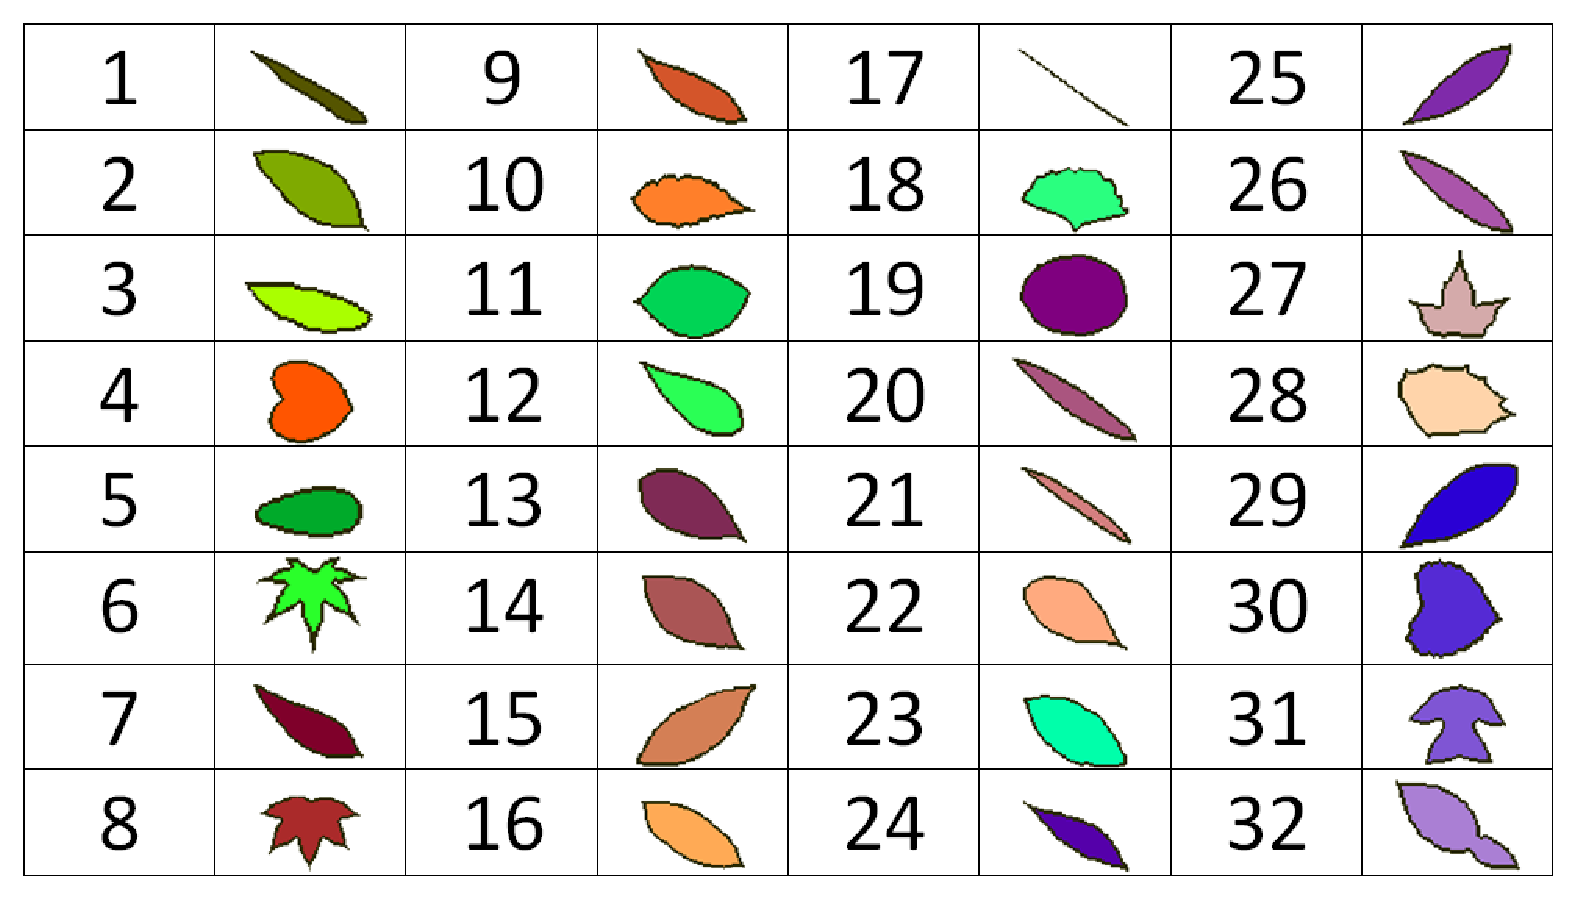
\includegraphics[width = 0.99\textwidth]{fig5.eps}
\caption{\label{fig:optimization_result} MDS projections of an experiment with $99$ shapes from Kimia data set \citep{Sebastian:2004}. The images display how clusters evolve during an optimization process (DE), as well as MAD and $R^2$ values.}
\end{figure}

The $R^2$ coefficient measures the fitness degree of the low-dimensional representation. This coefficient indicates, in percentage, the fitness of a model to the observed data. Thus, the closer the value of $R^2$ is to 1, the better the model fits the observed data. 

Let $d$ and $\hat{d}$ be the symmetrical distance matrices between feature vectors in the low and high-dimensional space. The $R^2$ coefficient is given by
\begin{equation}
R^2= 1-\frac{\sum_{i=1}^n \sum_{j = i}^{n}(\hat{d}_{i,j} - d_{i,j})^2}{\sum_{i=1}^n\sum_{j=i}^n (d_{i,j}-\bar{d})^2}
\text{,}\:\: R^2 \in [0,1]
\end{equation}

\noindent where $n$ is the number of samples, $d_{i,j}$ the distance between samples $i$ and $j$ in the high-dimensional space, $\hat{d}_{i,j}$ the distance between samples $i$ and $j$ in the low-dimensional space and $\bar{d}$ the mean distance in the high-dimensional space.

The MDS projections in Figure \ref{fig:optimization_result} illustrate how the shape clusters evolve as DE searches for the  optimized parameters of the shape descriptor (NMBE). The shape samples are from Kimia data set \cite{Sebastian:2004} which comprises $99$ shape images. Here, we have employed a manifold learning technique to produce the MDS projections of the optimized NMBE via DE. Figure \ref{fig:optimization_result} also shows that when the MAD values decreased, the inter-class distances increased and therefore the shape clusters became more evident.  At the minimum value of MAD, i.e., when the optimization process converged, the only clusters that were not well separated were the four-legged animals and the hand shapes. 

\end{comment}
